\documentclass[10pt,aspectratio=149]{beamer}
\usecolortheme{Calm}
\usetheme{Calm}
%\usefonttheme[onlymath]{serif} % beamer force les maths en cmss par défaut, qui n'a pas de vrai gras : \mathbf{} restait fin
\usepackage{amsmath}
\usepackage{pgfplots}
\pgfplotsset{compat=1.18}
\usepackage{pgfplotstable}
\usepackage[utf8]{inputenc}
\usepackage{hyperref}
\RequirePackage[absolute,overlay]{textpos}
%\usepackage[sfdefault]{cabin}
%\usepackage[T1]{fontenc}
%\setlength{\TPHo{}rizModule}{\paperwidth}
%\setlength{\TPVertModule}{\paperheight}
%\definecolor{OQEdarkblue}{HTML}{046085}


\defbeamertemplate*{background canvas}{bg}
{%
  \color{lightgray!40}\vrule width\paperwidth height\paperheight% added bg color
}

% Centered, larger display equation
\newcommand{\keyeq}[1]{%
  \begin{center}
    \Large$\displaystyle #1$
  \end{center}%
}

% Same style, for a system of equations aligned on "="
% (rows separated by \\, each row written as LHS &= RHS)
\newcommand{\keyeqs}[1]{%
  \begin{center}
    \normalsize$\displaystyle
    \begin{aligned}
    #1
    \end{aligned}
    $
  \end{center}%
}

%------------------------------

\author{Dominique Gravel}
\title{A spatial perspective on the stability-complexity relationship}
\date{August 27th, 2026}
\institute{Université de Sherbrooke \\ Summer school in biodiversity modelling}

%------------------------------
% TITLE SLIDE
%------------------------------

\usebackgroundtemplate
{
  
\includegraphics[width=\paperwidth,height=\paperheight]{bg}%
}

\begin{document}

	\begin{frame}[plain]
		\titlepage
	\end{frame}

%------------------------------
% INTRO
%------------------------------

\begin{frame}{An old and intuitive interpretation}
	    
	For decades, a dominant paradigm was that complex communities are more stable (Odum 1953; MacArthur 1955; Elton 1958; Hutchinson 1959).\\

	\vskip 3em

	MacArthur (1955) stated very generally that \alert{"a larger number of paths through each species is necessary to reduce the effects of overpopulation of one species"}. He later concluded that\alert{"stability increases as the number of links increases"}.
	
	\end{frame}

%------------------------------

	\begin{frame}{But....}
		\begin{columns}
			\begin{column}{0.5\textwidth}
				\begin{center}
					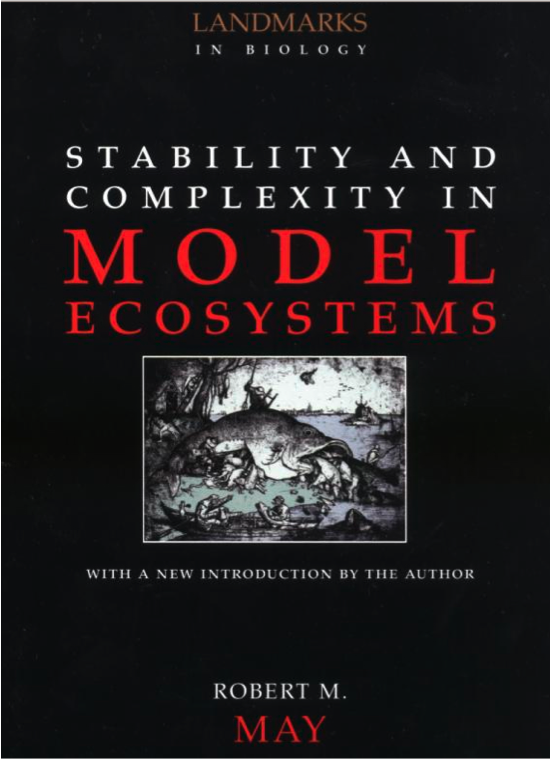
\includegraphics[height=0.65\textheight]{Figs/May_book}
				\end{center}
			\end{column}
%----
			\begin{column}{0.5\textwidth}
				\begin{center}
					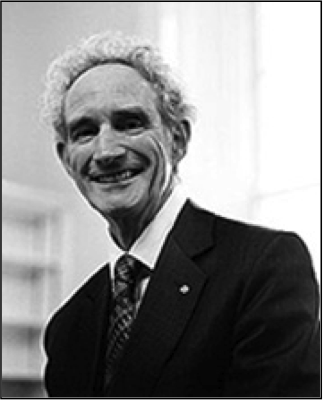
\includegraphics[height=0.45\textheight]{Figs/May_picture}
				\end{center}
			\end{column}
		\end{columns}	    	
	\end{frame}

%------------------------------

	\begin{frame}{Stability of random ecosystems}
		\begin{columns}
			\begin{column}{0.5\textwidth}
				\begin{center}
					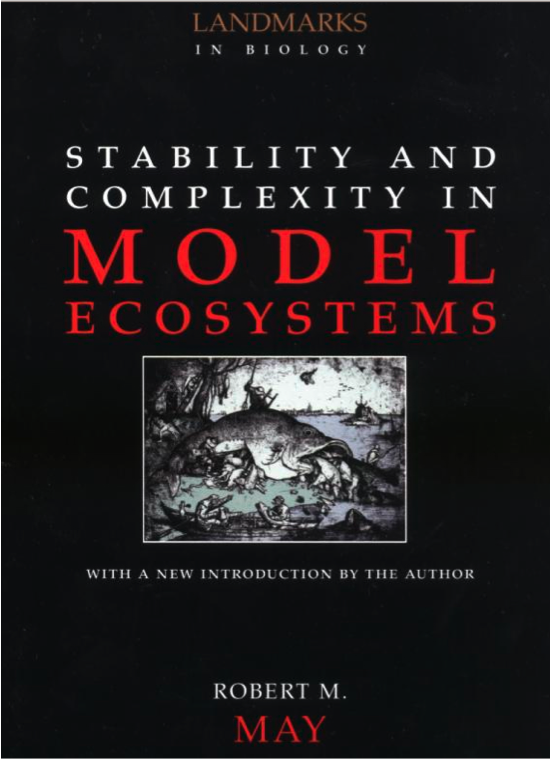
\includegraphics[height=0.65\textheight]{Figs/May_book}
				\end{center}
			\end{column}
%----
			\begin{column}{0.5\textwidth}
				\[ J = 
				\begin{bmatrix}
                    - & + & 0 & 0 & - \\
                    0 & - & 0 & 0 & 0 \\
					0 & - & - & 0 & 0 \\
					- & 0 & 0 & - & - \\
					0 & 0 & + & 0 & -
				\end{bmatrix} \] 
			\end{column}
		\end{columns}	    	
	\end{frame}

%------------------------------

	\begin{frame}{Stability of random ecosystems}
		\begin{columns}
			\begin{column}{0.5\textwidth}

				Criteria for local stability of complex random ecosystems:

				\keyeqs{\alpha\sqrt{SC}<1}

				Where: 
				\begin{itemize}
					\item $\alpha$: standard deviation of non null elements of the Jacobian
					\item $S$: species richness
					\item $C$: Connectance
				\end{itemize}
			\end{column}
%----
			\begin{column}{0.5\textwidth}
				\[ J = 
				\begin{bmatrix}
                    - & + & 0 & 0 & - \\
                    0 & - & 0 & 0 & 0 \\
					0 & - & - & 0 & 0 \\
					- & 0 & 0 & - & - \\
					0 & 0 & + & 0 & -
				\end{bmatrix} \] 
			\end{column}
		\end{columns}	    	
	\end{frame}

%------------------------------

	\begin{frame}{The complexity paradox}
	    
		\begin{center}
			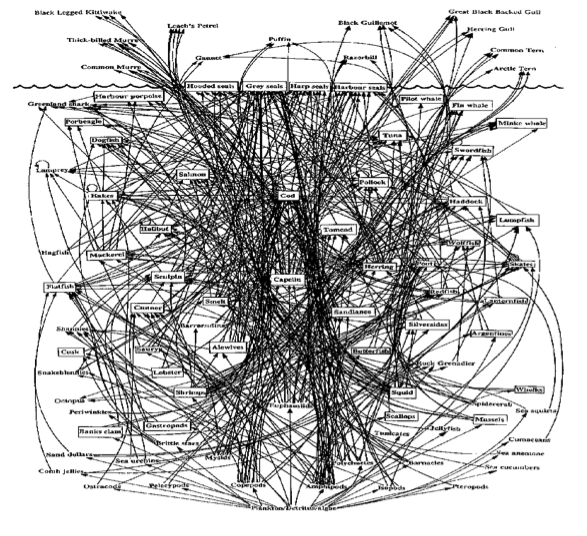
\includegraphics[height=0.75\textheight]{Figs/cod_web}
		\end{center}
	
	\end{frame}

%------------------------------

	\begin{frame}{Food webs are not random}
	    
		\begin{columns}
			\begin{column}{0.5\textwidth}			
				Pimm, S.L. (1982). Food Webs. University of Chicago Press. Chicago.

				\begin{itemize}
					\item Food webs are not random
					\item There are multiple meanings to stability
				\end{itemize}
			\end{column}
%----
			\begin{column}{0.5\textwidth}
				\begin{center}
					
\includegraphics[height=0.65\textheight]{Figs/pimm_book}
				\end{center}
			\end{column}
		\end{columns}	    	
	
	\end{frame}

%------------------------------

\begin{frame}{Testing scaling relationships}
	    
	\begin{columns}
		\begin{column}{0.5\textwidth}			

			Given the relationship

			\keyeqs{\alpha\sqrt{SC}=\alpha\sqrt{\frac{L}{S}}<1}

			We should find a relationship between L and S, such that:
			\keyeqs{log(L) = \frac{1}{2}log(\alpha) + log(S)}

		\end{column}
%----
		\begin{column}{0.5\textwidth}
			\begin{center}
				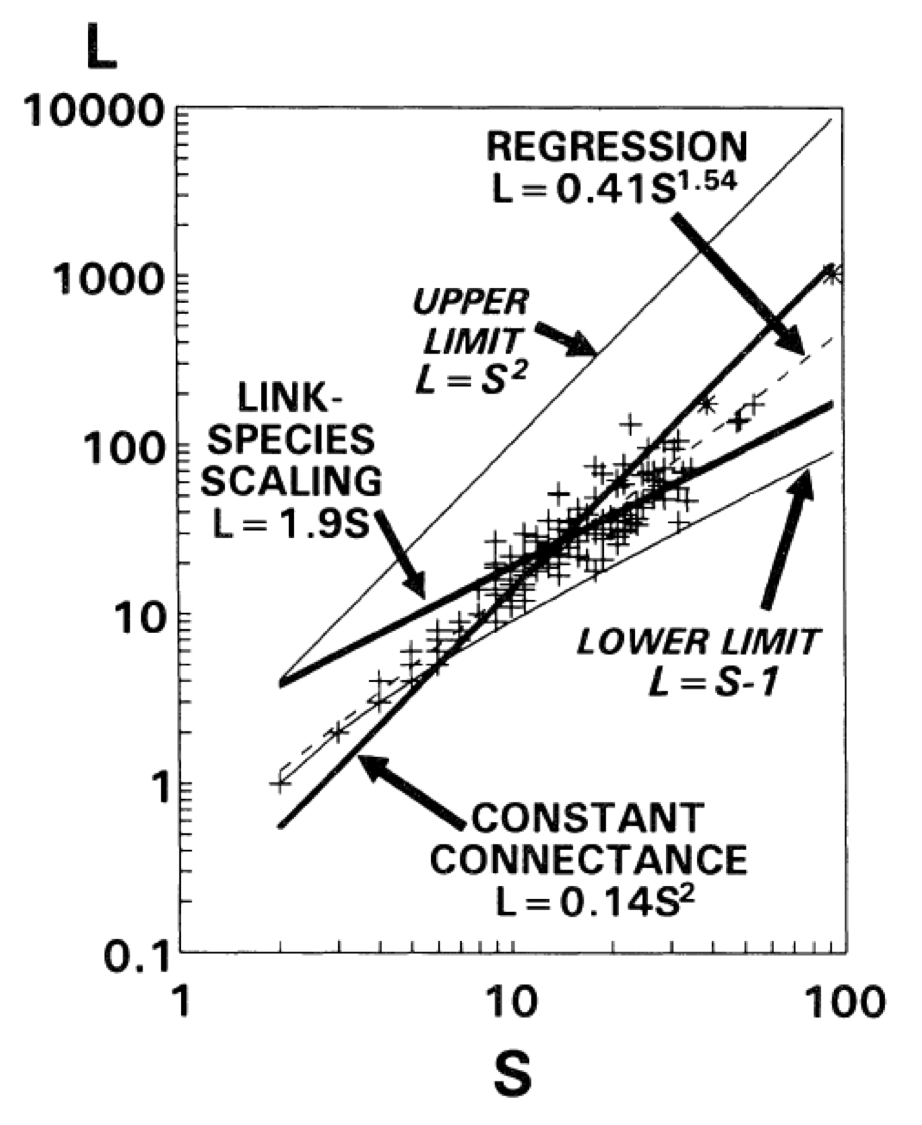
\includegraphics[height=0.65\textheight]{Figs/link_scaling}
			\end{center}
		\end{column}
	\end{columns}	    

\end{frame}

%------------------------------

\begin{frame}{And interactions are not normally distributed}
	
	\begin{columns}
		\begin{column}{0.4\textwidth}			
			What about the $\alpha$ parameter?\\

		\end{column}
%----
		\begin{column}{0.6\textwidth}
			\begin{center}
				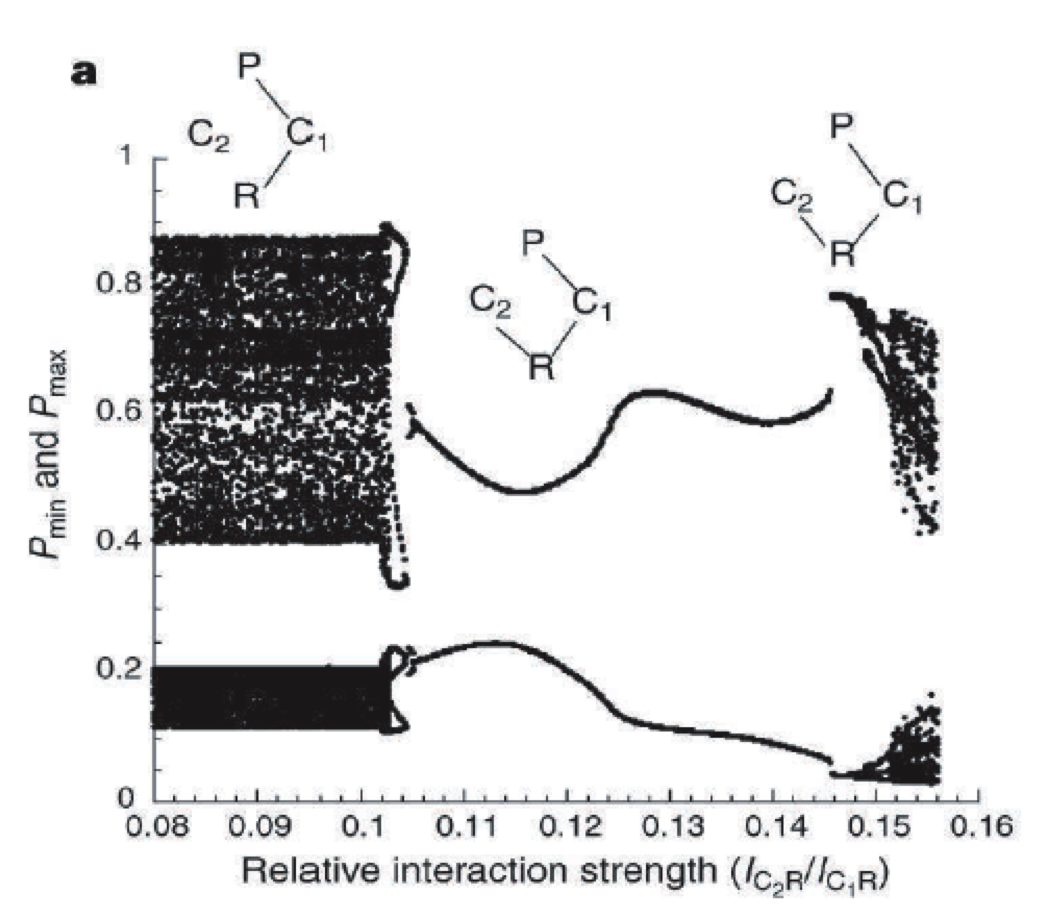
\includegraphics[height=0.7\textheight]{Figs/mccann}\\
				\footnotesize McCann et al. 1998. Nature.
			\end{center}
		\end{column}
	\end{columns}	    

\end{frame}

%------------------------------

\begin{frame}{And interactions are not normally distributed}
	
	\begin{columns}
		\begin{column}{0.4\textwidth}			
			What about the $\alpha$ parameter?\\
			
		\end{column}
%----
		\begin{column}{0.6\textwidth}
			\begin{center}
				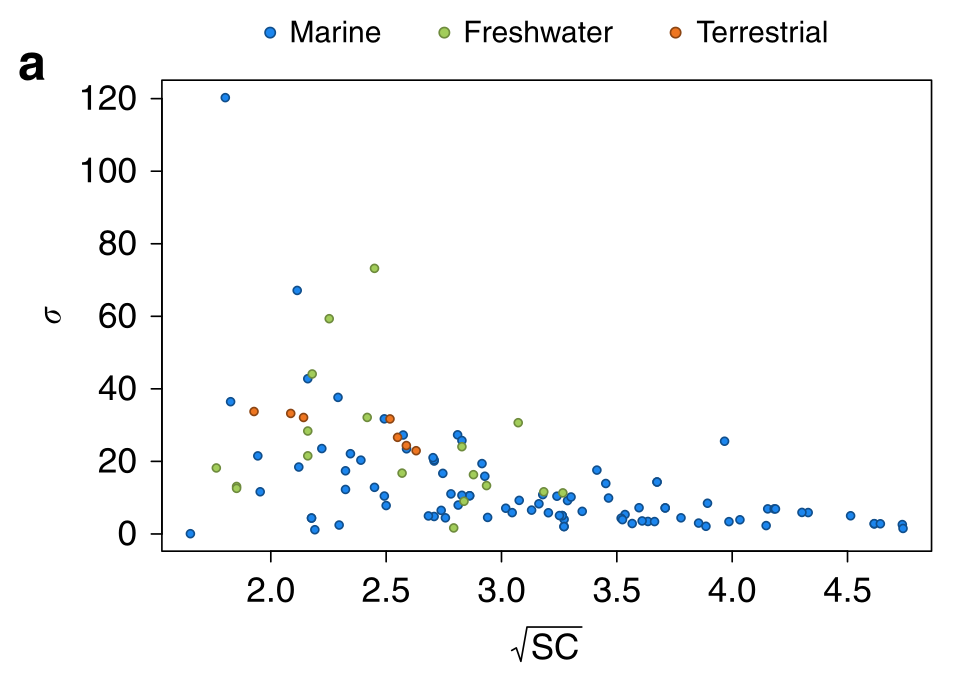
\includegraphics[height=0.5\textheight]{Figs/jacquet2016}\\
				\footnotesize Jacquet et al. 2016. Nat. Communications
			\end{center}
		\end{column}
	\end{columns}	    

\end{frame}

%------------------------------
% DIFFUSION EXERCISE
%------------------------------

{
\usebackgroundtemplate{}
\begin{frame}

	\pagecolor{BDQC1st}
	\color{white}

	\LARGE{\textit{But what about spatial dynamics ?}}

\end{frame}
}

%------------------------------

\begin{frame}{Rosenzweig-MacArthur consumer-resource model}


	Resource dynamics follow a logistic growth, minus consumption : 
		\keyeqs{\frac{dR}{dt} = rR*(1-\frac{R}{K}) - \frac{aRC}{1+bR}}

	And consumer dynamics simply transform consumption into biomas, minus mortality :
		\keyeqs{\frac{dC}{dt} = \frac{eaRC}{1+bR}-mC}

	You can solve the equation at equilibrium by setting differential equations to 0 and isolating the two variables. 

\end{frame}

%------------------------------

\begin{frame}{Rosenzweig-MacArthur predator-prey model}{Paradox of enrichment}

	\begin{center}
		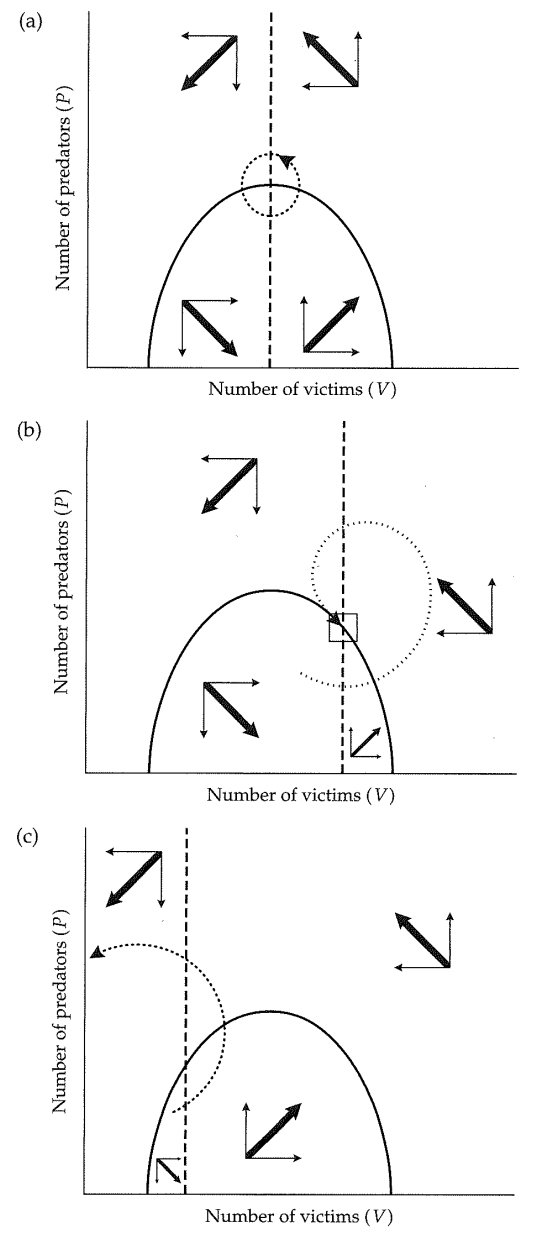
\includegraphics[height=0.75\textheight]{Figs/paradox}
	\end{center}

\end{frame}

%------------------------------

\begin{frame}{Rosenzweig-MacArthur predator-prey model}{Adding resource immigration}

	Resource immigration is stabilizing because it induces indirect density-dependence : 

		\keyeqs{\frac{dR}{dt} = rR*(1-\frac{R}{K}) - \frac{aRC}{1+bR} + I}

	Or : 

		\keyeqs{\frac{dR}{dt}\frac{1}{R} = r(1-\frac{R}{K}) - \frac{aC}{1+bR} + \frac{I}{R}}

\end{frame}

%------------------------------

\begin{frame}{Rosenzweig-MacArthur predator-prey model}{Adding consumer immigration}

	In the situation where : 

		\keyeqs{\frac{dC}{dt} = \frac{eaRC}{1+bR}-mC + I} 

	And we find that increasing $I$

	\begin{itemize}
		\item Drives the resource towards extinction
		\item Generates indirect density-dependence, which is also stabilizing
	\end{itemize}

\end{frame}

%------------------------------

\begin{frame}{Rosenzweig-MacArthur predator-prey model}{Discrete landscale}

	Consider a two patch system : 

		\keyeqs{\frac{dR_x}{dt} = rR_x*(1-\frac{R_x}{K}) - \frac{aR_xC_x}{1+bR_x} - d_R R_x + d_R (R_{x-1}+R_{x+1})/2}

	And 

		\keyeqs{\frac{dC_x}{dt} = \frac{eaR_xC_x}{1+bR_x}-mC_x - d_C C_x + d_c (C_{x-1}+C_{x+1})/2} 	

\end{frame}

%------------------------------

\begin{frame}{Rosenzweig-MacArthur predator-prey model}{Discrete landscape}

	\begin{itemize}
		\item Implement the model over a large one dimensional lattice, without diffusion
		\item Extract and plot time series
		\item Tune parameters to get close to instability
		\item Add progressively the resource and consumer diffusion parameters
		\item \textbf{Advanced} : add spatial variability in $K$ and compare results
	\end{itemize}

\end{frame}

%------------------------------

\begin{frame}{From local to regional dynamics}
	    
	\begin{center}
		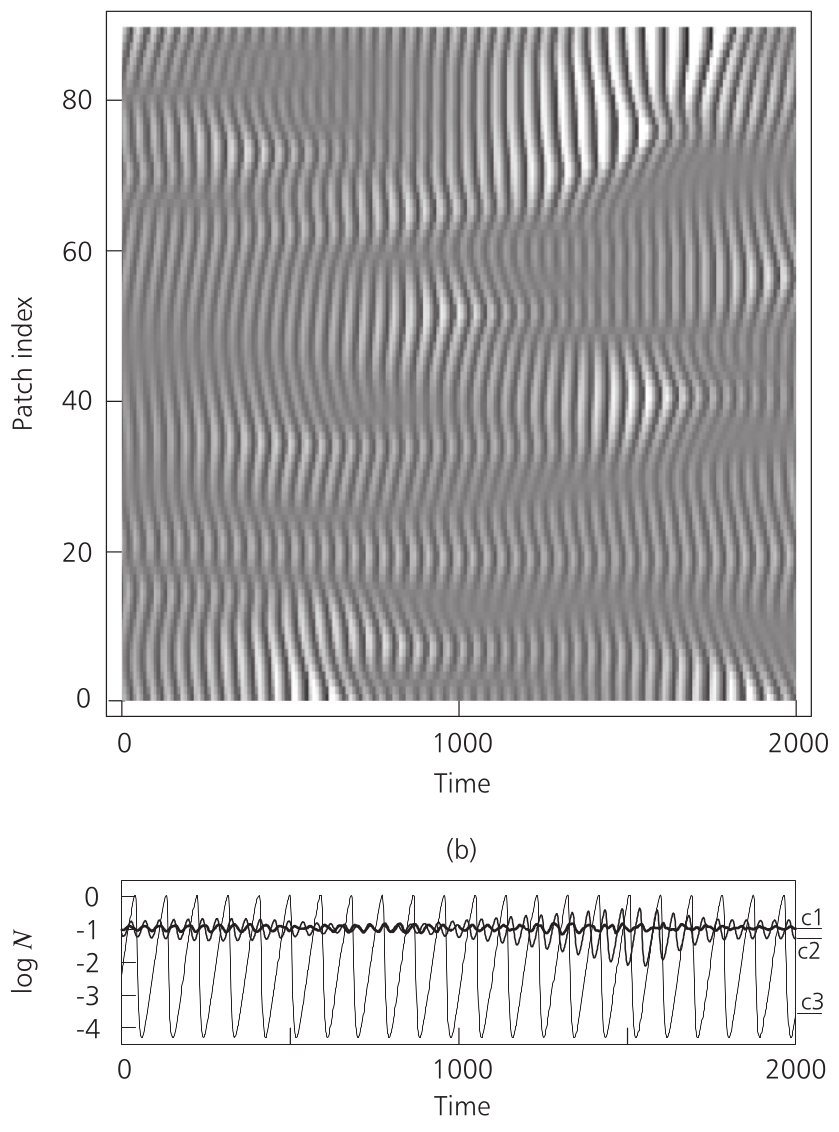
\includegraphics[height=0.75\textheight]{Figs/jansen2000}\\
		\footnotesize Jansen et al. 2000
	\end{center}

\end{frame}

%------------------------------
% Stability-complexity theory
%------------------------------

{
\usebackgroundtemplate{}
\begin{frame}

	\pagecolor{BDQC1st}
	\color{white}

	\LARGE{\textit{Stability and complexity in random metaecosystems}}

\end{frame}
}

%------------------------------

\begin{frame}{From local to regional dynamics}
	    
	\begin{center}
		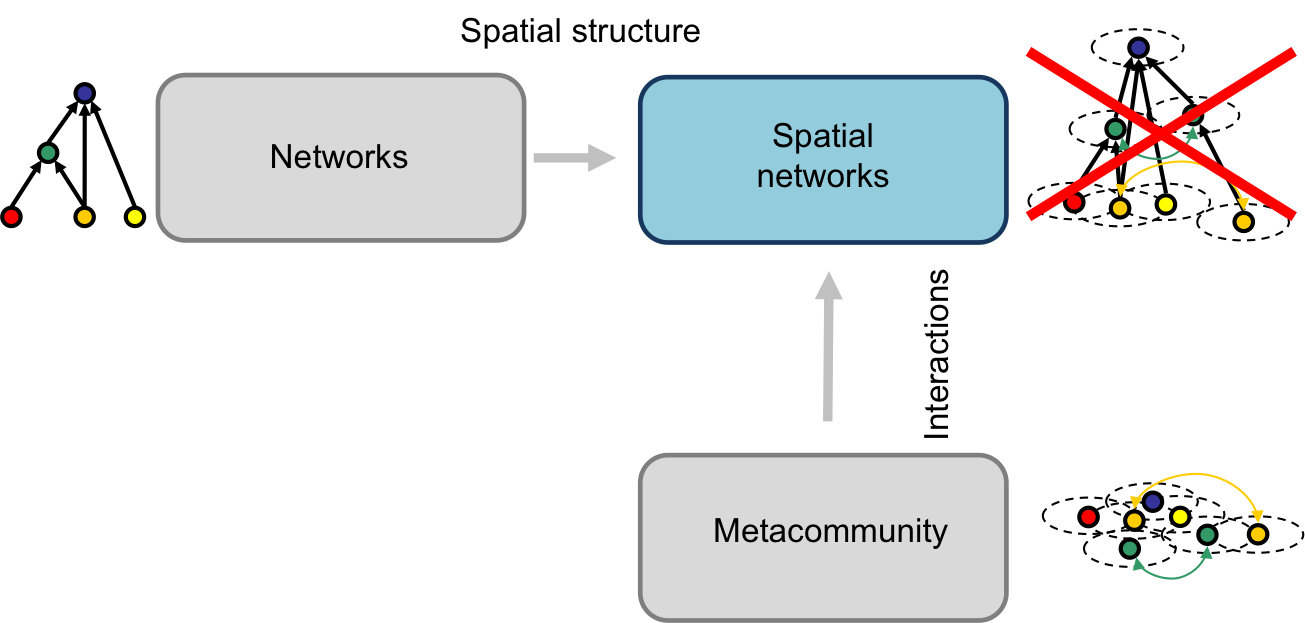
\includegraphics[height=0.55\textheight]{Figs/spatial_networks}
	\end{center}

\end{frame}

%------------------------------

\begin{frame}{Jacobian matrices in space}

	\begin{columns}
		\begin{column}{0.4\textwidth}			
			What's happening with spatialization?
			\begin{itemize}
				\item The number of equations increases
				\item Connectance decreases
				\item We don't know what's happening with $\alpha$
			\end{itemize}
		\end{column}
		%----
		\begin{column}{0.7\textwidth}
			\begin{center}
				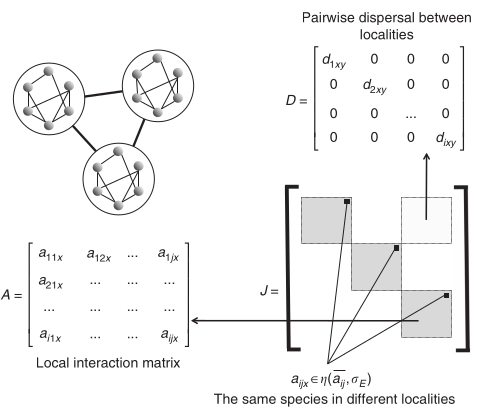
\includegraphics[height=0.6\textheight]{Figs/gravel2016a}\\
				\footnotesize Gravel et al. 2016. Nat. Communications
			\end{center}
		\end{column}
	\end{columns}	 

\end{frame}

%------------------------------

\begin{frame}{Jacobian matrices in space}

	\begin{columns}
		\begin{column}{0.4\textwidth}			
			Two problems:
				\begin{enumerate}
					\item Stability of the equilibrium
					\item Feasability of the equilibrium
				\end{enumerate}
		\end{column}
		%----
		\begin{column}{0.7\textwidth}
			\begin{center}
				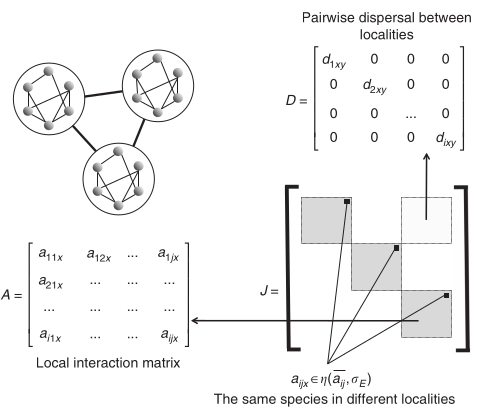
\includegraphics[height=0.6\textheight]{Figs/gravel2016a}\\
				\footnotesize Gravel et al. 2016. Nat. Communications		
			\end{center}
		\end{column}
	\end{columns}	 

\end{frame}

%------------------------------

\begin{frame}{Analytical results}

	\begin{center}
		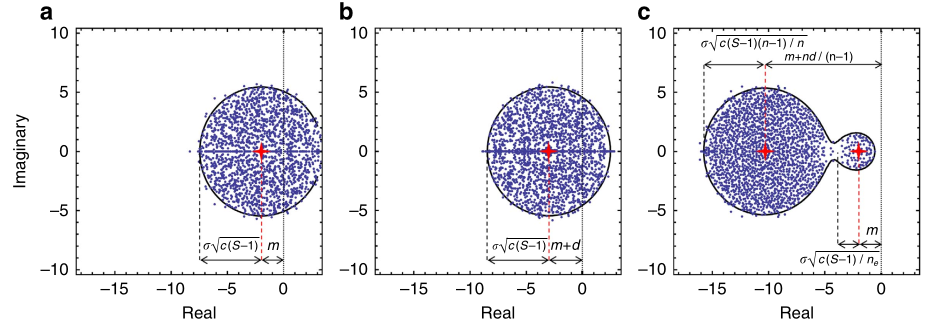
\includegraphics[height=0.45\textheight]{Figs/gravel2016b.png}\\
		\footnotesize Gravel et al. 2016. Nat. Communications						
	\end{center}

	Spatial structure and diffusion
	\begin{itemize}
		\item Move the center of the disk toward the left 
		\item Reduce the radius of the disk 
	\end{itemize}
\end{frame}

%------------------------------

\begin{frame}{And the feasibility problem}{Diffusion and environment}

	\begin{columns}
		\begin{column}{0.3\textwidth}			
			\begin{itemize}
				\item Indirect density-dependence
				\item Source-sink dynamics
				\item Feasibility
			\end{itemize}
		\end{column}
		%----
		\begin{column}{0.7\textwidth}
			\begin{center}
				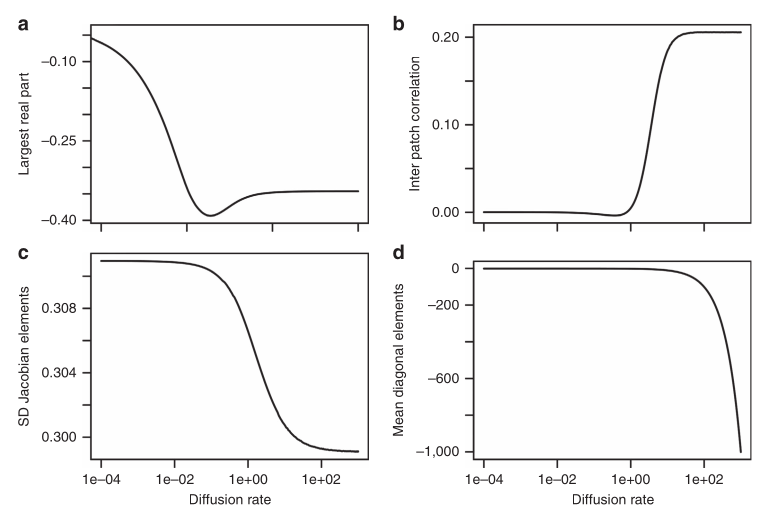
\includegraphics[height=0.6\textheight]{Figs/gravel2016c}\\
				\footnotesize Gravel et al. 2016. Nat. Communications		
			\end{center}
		\end{column}
	\end{columns}	 

\end{frame}

%------------------------------
% CONCLUSION
%------------------------------

{
\usebackgroundtemplate{}
\begin{frame}

	\pagecolor{BDQC1st}
	\color{white}

	\LARGE{\textit{Conclusion}}

\end{frame}
}

%------------------------------

\begin{frame}{Stability and complexity}{Spatial dynamics}

	\begin{columns}
		\begin{column}{0.5\textwidth}			
			\begin{itemize}
				\item Food webs are not random
				\item Spatial structure influence stability
				\item Distinct spatial rates leads to funky dynamics
				\item What's the value of this theory to the field ... 
			\end{itemize}
		\end{column}
	%----
		\begin{column}{0.5\textwidth}
			\begin{center}
				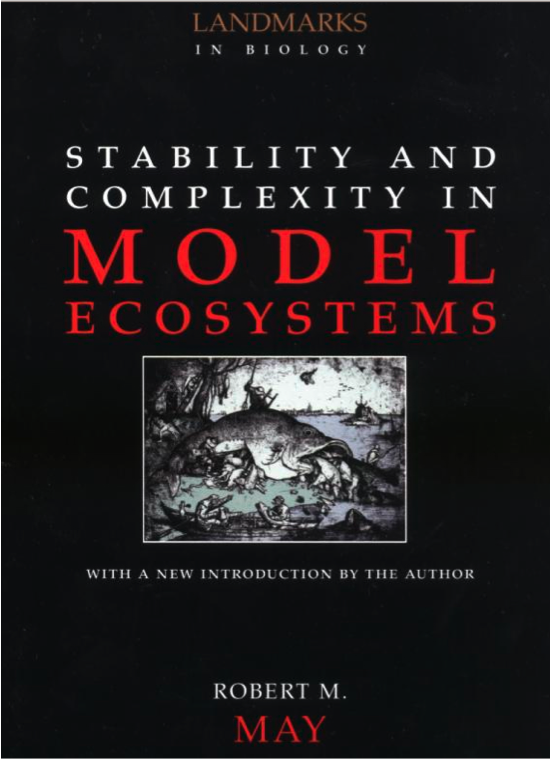
\includegraphics[height=0.65\textheight]{Figs/May_book}
			\end{center}
		\end{column}
	\end{columns}	    

\end{frame}
%------------------------------
%------------------------------
%------------------------------
\end{document}
